\section{Motivation}
\begin{frame}
  \frametitle{rECGA}
  \vspace*{-28pt}
  \begin{itemize}
    \item Discretization 
      \begin{itemize}
        \item Continuous domain $\rightarrow$ Discrete domain $\rightarrow$
          Continuous domain
        \item Is there any distortion?
      \end{itemize}
  \end{itemize}
  \vspace*{-23pt}
  \begin{figure}[htpb]
    \flushright
    \includegraphics[bb= 92 397 755 220, clip, width=0.5\textwidth]{Discretization.eps}
  \end{figure}
  \vspace*{28pt}
  \begin{itemize}
    \item Unreasonable sampling
      \begin{itemize}
        \item cliff between each bin is sometimes steep.
      \end{itemize}
      \vspace{-14pt}
  \begin{figure}[hpb]
    \includegraphics[bb = 67 546 774 21,clip, width = 0.3\textwidth]{Sampling.eps}
  \end{figure}
\end{itemize}

\end{frame}


\begin{frame}{rECGA}
  \begin{itemize}
    \item rECGA tackles the difficulty of
      and \alert{Ill-conditioned}.
      \vspace*{14pt}
    \item rECGA limits the searching region in early stage to deal with
      \alert{dimensionality}.
      \vspace*{14pt}
    \item rECGA struggles in exploration and encounters the previously
      introduced difficulties.
      \vspace*{14pt}
    \item Why not make real-valued problem solved by methods encoded in
      continuous domain?

  \end{itemize}
\end{frame}
\begin{frame}{CMA-ES}
  \begin{itemize}
    \item An outstanding local optimizer
    \item Tackles \alert{non-separable} by maintaining a
      covariance matrix
    \item Usually encounters premature convergence
  \end{itemize}
  \begin{figure}[htpb]
    \centering
    \vfill\includegraphics[scale = 0.3]{LocalOptima.eps}
  \end{figure}
\end{frame}
\begin{frame}{Hypothesis}
  \begin{itemize}
    \item Both CMA-ES and rECGA suffer from \alert{ruggedness} for
      insufficient exploration.
      \vspace*{8pt}
    \item What if there is implicit information between local optima?
    \item We are interested in rugged problems with implicit tendency
  \end{itemize}
  \vspace*{10pt}
  \begin{figure}[hp]
    \centering
    \includegraphics[scale=0.3]{Problem.eps}
  \end{figure}
\end{frame}

\begin{frame}{Hypothesis}
  \begin{itemize}
    \item Assume problems are with such structure
      \vspace*{10pt}
    \item We are aiming to fetch more promising region by evolving the
      tendency
  \end{itemize}
  \vspace*{10pt}
  \begin{figure}[hp]
    \centering
    \includegraphics[scale=0.3]{tendency.eps}
  \end{figure}
\end{frame}
\begin{frame}{Hypothesis}
  \begin{itemize}
    \item A reasonable discretization 
      \vspace*{10pt}
    \item Clustering based on space locality  
  \vspace*{10pt}
\item Performing a 2nd layer CMA-ES for evolving the tendency
  \end{itemize}
  \vspace*{10pt}
  \begin{figure}[htpb]
    \centering
    \includegraphics[scale=0.35]{hypothesis_discretization.eps}
  \end{figure}
\end{frame}

\begin{frame}{Expected benefit}
  \begin{itemize}
    \item A soft, adaptive discretization
      \begin{itemize}
        \item Iteratively exploring better regions.
        \item Generated regions are also source for better regions.
      \end{itemize}
      \vspace*{14pt}
    \item Each region can be highly exploited. 
      \begin{itemize}
        \item 1st layer CMA-ES quickly outputs local optimum.
      \end{itemize}
  \end{itemize}
\end{frame}




%\begin{frame}{Hypothesis}
%
%  \begin{itemize}
%    \item Increasing diversity by maintaining multiple groups.
%      \begin{itemize}
%        \item kind of discretization.
%        \item How to define the number of groups?
%        \item What is the criteria for individuals to form a group?
%      \end{itemize}
%      \vspace*{14pt}
%    \item There is implicit information hidden between groups.
%      \begin{itemize}
%        \item How to extract the information?
%        \item How to benefit from the information and obtain
%          better solutions?
%          \begin{itemize}
%            \item Inspired by discretization, we aim to find a more
%              promising region.
%          \end{itemize}
%      \end{itemize}
%      \vspace*{14pt}
%    \item 2-layer CMA-ES is introduced
%      \begin{itemize}
%        \item Inner layer for exploitation
%        \item Outer layer for exploration
%      \end{itemize}
%  \end{itemize}

%\end{frame}
